\chapter{Quantum systems}
    In this chapter we'll discuss different quantum systems which will be
    explored.
    We'll discuss how we represent a general quantum system via the Python class
    \pyth{QuantumSystem} and the methods that this class incorporates.
    Before delving into the mathematics of quantum dots, and atoms and
    molecules, we will discuss what we want from our basis sets.
    \begin{enumerate}
        \item For all types of calculations we need access to the one- and
            two-body matrix elements of the Hamiltonian, and potentially the
            nuclear repulsion energy.
            That is, we need to find values for $\oneten^{p}_{q}$ and
            $\twoten^{pq}_{rs}$.
            In case of a non-orthonormal basis set we also need the overlap
            matrix $\overlapten^{p}_{q}$.
        \item For time-evolution using a dipole laser we need the dipole matrix
            elements $\vfg{d}^{p}_{q}$.
        \item For visualization of the particle density we need the
            single-particle states.
    \end{enumerate}
    If our only interest is the ground state energy, we can get far with point 1
    listed above.
    However, for us to include interaction with a laser field we also need the
    dipole matrix elements as we are working in the dipole approximation.
    The single-particle states are necessary for visualization of the system on
    a grid either via the particle density or by themselves.
    We will visualize some of our systems to get a qualitative description of
    what we are looking at, but often we are more interested in quanitifying our
    results and they single-particle states are not necessarily needed.
    That is, they are of course needed when computing the integrals for the
    matrix elements, but an explicit evaluation of the single-particle states on
    a grid is not always necessary.
    The Python class \pyth{QuantumSystem} therefore builds the basis sets and
    serves as a container of sorts with the necessary matrix elements listed
    above.

    Often the limitation of basis sets comes from the calculation of the
    two-body matrix elements as these integrals will in many cases be the
    bottleneck.
    This is the reason why we choose systems with closed form solutions to the
    most intensive integrals, and then do a basis transformation using the
    variational method, and eventually Hartree-Fock to build more complicated
    systems.
    As part of this thesis we have implemented several systems, they are:
    \begin{enumerate}
        \item The one-dimensional quantum dot on a grid supporting arbitrary
            one-dimensional potentials.
        \item The two-dimensional quantum dot in a harmonic oscillator, in a
            sharp double well, in a smooth double well, and subject to a
            magnetic field.
    \end{enumerate}
    In this thesis we will look at the one-dimensional quantum dot, and briefly
    at the two-dimensional quantum dot in a harmonic oscillator trap.
    The remaining potentials for the two-dimensional quantum dot are discussed
    in the thesis by \citeauthor{greg-winther} \cite{greg-winther}.
    However, we will discuss the implementation of some of these systems as they
    constituted a large part of this thesis.

    We will in this thesis mainly concern ourselves with atoms and molecules.
    The subject of atomic and molecular basis sets is a vast one, and we've not
    had the luxury of implementing these systems ourselves.
    We've instead implemented an interface towards the existing libraries PySCF
    \cite{pyscf} and Psi4 \cite{psi4} in order to get access to good and
    efficient basis sets for atoms and molecules.


    \section{One-dimensional quantum dots}
    \label{sec:one-dim-qd}
    Artificial atoms, or the so-called quantum dots, constitute a hot topic in
    condensed matter physics and material sciences. We will be exploring
    several types of quantum dots in both one and two dimensions in this
    thesis. The difference between the types of quantum dots is found in the
    one-body potential. All of the dots share the characteristic of being in an
    infinite well which makes the systems \emph{bound}. In our study of systems
    subject to intense laser fields, this will prove to be a bad approximation
    when the laser becomes very strong as the particles have no way of being
    ionized, i.e., escape the potential well.  Even so, for weak laser fields
    and for ground state calculations, they serve as excellent candidates for
    our methods.
    % TODO: This text needs some work

    The time-independent one-dimensional quantum dot can be described by the
    one-body Hamiltonian
    \begin{align}
        \oneten(x)
        = -\frac{\hslash^2}{2m} \dod[2]{}{x}
        + v(x),
        \label{eq:one-body-odqd}
    \end{align}
    where $v(x)$ is a potential function.
    In one dimension it is quite cheap to define a grid and use finite
    differences to solve the one-dimensional Schrödinger equation.
    Furthermore, for the systems we explore, numerically solving the Coulomb
    integrals is also feasible.
    This solution has its drawbacks in that we approximate an infinite integral
    on a finite line, but it also has the advantage of being ``blind'' to the
    choice of potential.
    This makes the solution completely general and opens up for a wide variety
    of potentials without the need for any extra mathematics.

    \subsection{Discretizing the one-dimensional quantum dot}
        \label{subsec:discretizing-the-odqd}
        For a given one-body Hamiltonian $h(x)$ on the form described in
        \autoref{eq:one-body-odqd}, we wish to find a solution the
        time-indepedent Schrödinger equation
        \begin{align}
            \oneten(x)\psi(x) = \epsilon \psi(x),
        \end{align}
        where we've ignored labels on the eigenpair $(\epsilon, \psi(x))$ for
        now to avoid clutter.
        However, do be aware that we are looking for a spectrum of eigenstate.
        We use the central finite difference scheme for the kinetic term in the
        one-body Hamiltonian, that is,
        \begin{align}
            \dod[2]{\psi(x)}{x}
            = \frac{
                \psi(x + \Delta x) - 2\psi(x) + \psi(x - \Delta x)
            }{(\Delta x)^2}
            + \mathcal{O}\para{(\Delta x)^2}.
        \end{align}
        Now we can write the time-independent Schrödinger equation in the fully
        discretized form
        \begin{align}
            \oneten(x) \psi(x)
            &= -\frac{1}{2}
            \frac{
                \psi(x + \Delta x) - 2\psi(x) + \psi(x - \Delta x)
            }{(\Delta x)^2}
            + v(x)\psi(x)
            = \epsilon \psi(x),
        \end{align}
        where we use the more convenient atomic units with $\hslash = m = 1$.
        Introducing the uniformly discretized grid $x_i$ where $i \in \brac{1,
        n}$ and $n$ is the number of grid points, we label the wave function by
        $\psi_i = \psi(x_i)$.
        We have that
        \begin{align}
            x_{i + 1} = x_i + \Delta x,
        \end{align}
        with $\Delta x$ being the step-size between the grid points.
        There exists smarter grid choices than the uniform grid, but for our
        simulations the uniform grid is quite good enough.
        Collecting the wave function evaluated at the same grid points in the
        time-independent Schrödinger equation we can write
        \begin{align}
            \oneten \psi_i
            &=
            \para{
                \frac{1}{(\Delta x)^2}
                + v_i
            }\psi_i
            - \frac{1}{2 (\Delta x)^2}
            \para{
                \psi_{i + 1}
                + \psi_{i - 1}
            }
            = \epsilon \psi_i.
        \end{align}
        We are now in a position to formulate this equation as a generalized
        eigenvalue equation on the form
        \begin{align}
            \vfg{\oneten}\vfg{\psi}
            = \vfg{\epsilon}\vfg{\psi},
            \label{eq:one-dim-qd-eigh}
        \end{align}
        where the one-body Hamiltonian matrix is a tridiagonal matrix with
        diagonal elements
        \begin{align}
            \oneten_{ii}
            =
            \frac{1}{(\Delta x)^2}
            + v_i
        \end{align}
        and off-diagonal elements
        \begin{align}
            \oneten_{ij}
            = -\frac{1}{2(\Delta x)^2}\para{
                \delta_{(i + 1) j}
                + \delta_{(i - 1) j}
            }.
        \end{align}
        Solving \autoref{eq:one-dim-qd-eigh} yields the full spectrum of
        $\vfg{h} \in \mathbf{C}^{n \times n}$ where $\vfg{\psi} \in
        \mathbf{C}^{n \times n}$ becomes a matrix with each column representing
        an eigenstate, and the rows the evaluation of the eigenstates on the
        grid.
        The quality of the eigenpairs is dependent on the number of grid points
        $n$, and ideally we should include many grid points such that $\Delta x
        \to 0$.
        However, we are not in a position to utilize all $n$ eigenstates in the
        later analysis and we will therefore truncate the number of orbitals to
        the number of basis functions $L$ that we wish to include.
        Furthermore, the systems we are exploring are spin-independent which
        means that we only use $L / 2$ orbitals from the spectrum of $\vfg{h}$,
        thus greatly reducing the number of single-particle functions.

        Depending on the scheme chosen for solving the generalized eigenvalue
        equation, one might need to normalize the eigenstates.
        Lastly, we have not discussed the boundary conditions for the
        eigenstates.
        We require that $\psi_p(-\infty) = \psi_p(\infty) = 0$.
        We can realize this by introducing two extra grid points $i = 0$ and $i
        = n + 1$ after we have diagonalized the one-body Hamiltonian matrix and
        set $\psi_p(x_0) = \psi_p(x_{n + 1}) = 0$.

        Having found the eigenpairs for the one-dimensional Hamiltonian, we
        construct a new, diagonal, one-dimensional Hamiltonian from the
        eigenenergies.
        The normalized eigenstates from the generalized eigenvalue equation will
        be orthonormal.


    \subsection{Constructing the dipole moments}
        The matrix elements of the dipole moment for the one-dimensional quantum
        dot is given by
        \begin{align}
            d_{pq}
            = \mel{\psi_{p}}{\position}{\psi_{q}}
            = \int_{-\infty}^{\infty}\dd x
            \psi^{*}_{p}(x) x \psi_{q}(x).
        \end{align}
        As we are using a grid based solution, we approximate this integral
        using a numerical integration scheme on the grid.
        In our implementation we use the trapezoidal rule.
        By defining
        \begin{align}
            f_{pq}(x) = \psi^{*}_{p}(x) x \psi_{q}(x),
        \end{align}
        and given a uniform grid for $x_i \in \brak{a, b}$ where $i \in \brac{1,
        n}$ such that $x_1 = a$ and $x_n = b$ with grid spacing $\Delta x$, we
        approximate the dipole elements by
        \begin{align}
            d_{pq}
            \approx
            \frac{\Delta x}{2}\sum_{i = 2}^{n}\brak{
                f_{pq}(x_{i}) + f_{pq}(x_{i - 1})
            }.
        \end{align}
        The reason for choosing the trapezoidal rule is for its ease of usage
        and implementation, as well as the method being quite fast and precise.
        It is however, not the best integrator there is and more precise
        solutions should be considered.
        % TODO: Explain the usage in numba


    \subsection{Integrating the Coulomb elements}
        The arguably heaviest computation in setting up a one-dimensional
        quantum dot system, is the Coulomb integrals.
        Still working with atomic units, we have $e = (4\pi \epsilon_0)^{-1} =
        1$ such that the Coulomb interaction can be represented by
        \begin{align}
            \twoten(x_i, x_j) = \frac{1}{\abs{x_i - x_j}}.
        \end{align}
        When integrating on a grid, we get numerical instabilities at the
        singularity when $x_1 = x_2$.
        This motivates the introduction of a \emph{shielded Coulomb interaction}
        \cite{suq, skattum2013time, kristiansen2017time} given by
        \begin{align}
            \twoten(x_i, x_j)
            &= \frac{\alpha}{\sqrt{(x_i - x_j)^2 + a^2}},
            \label{eq:shielded-coulomb}
        \end{align}
        where $\alpha$ is a dimensionless constant and the screening parameter
        $a$ removes the singularity without ruining the asymptotic behavior
        when $(x_i - x_j) \to \infty$ \cite{suq, kristiansen2017time}.

        The integral we wish to solve is then
        \begin{align}
            \mel{\psi_{p}\psi_{q}}{\twohamil}{\psi_{r}\psi_{s}}
            &=
            \int\dd x_1 \dd x_2
            \psi^{*}_{p}(x_1)\psi^{*}_{q}(x_2)
            \twoten(x_1, x_2)
            \psi_{r}(x_1)
            \psi_{s}(x_2),
        \end{align}
        where $\twoten(x_1, x_2)$ is the shielded Coulomb interaction.
        We introduce the inner integral $W_{qs}(x_1)$ given by
        \begin{align}
            W_{qs}(x_1)
            &= \int\dd x_2
            \psi^{*}_{q}(x_2) \twoten(x_1, x_2)
            \psi_{s}(x_2),
        \end{align}
        that is, we integrate over one of the two spatial integrals in the
        Coulomb interaction.
        We can thus write the Coulomb elements as
        \begin{align}
            \mel{\psi_{p}\psi_{q}}{\twohamil}{\psi_{r}\psi_{s}}
            &=
            \mel{\psi_{p}}{\hat{W}_{qs}}{\psi_{r}}
            =
            \int\dd x_1
            \psi^{*}_{p}(x_1)
            W_{qs}(x_1)
            \psi_{r}(x_1),
        \end{align}
        where we compute the inner integral $W_{qs}(x_1)$ on the entire grid
        initially.
        Defining the function $g_{qs}(x_i, x)$ to be
        \begin{align}
            g_{qs}(x_i, x) = \psi^{*}_{q}(x) \twoten(x_1, x) \psi_s(x),
        \end{align}
        we can compute the inner integrals using the trapezoidal rule in the
        samme manner as for the dipole elements.
        That is, for a given point $x_i$ we have
        \begin{align}
            W_{qs}(x_i)
            \approx \frac{\Delta x}{2}
            \sum_{j = 2}^{n}
            \brak{
                g_{qs}(x_i, x_j) + g_{qs}(x_i, x_{j - 1})
            }.
        \end{align}
        From this we can compute the Coulomb element by
        \begin{align}
            \mel{\psi_{p}\psi_{q}}{\twohamil}{\psi_{r}\psi_{s}}
            \approx
            \frac{\Delta x}{2}
            \sum_{i = 2}^{n}
            \brak{
                h^{pq}_{rs}(x_i) + h^{pq}_{rs}(x_{i - 1})
            },
        \end{align}
        where we've defined the function
        \begin{align}
            h^{pq}_{rs}(x_i)
            = \psi^{*}_{p}(x_i) W_{qs}(x_i) \psi_{r}(x_i).
        \end{align}
        Again, we emphasize that the choice of using the trapezoidal rule is
        based on convenience and can be replaced by a better integrator if it
        turns out that the integrals are too erroneous.


    \subsection{One-dimensional harmonic oscillator}
        The one-dimensional harmonic oscillator is usually one of the first
        models studied in undergraduate quantum mechanics courses.
        The one-body Hamiltonian of the one-dimensional harmonic oscillator is
        given by
        \begin{align}
            \onehamil = \frac{\momentum^2}{2m} + \half m\omega^2 \position^2,
            \label{eq:1dho-hamiltonian}
        \end{align}
        where the latter term, i.e., the one-body potential, gives rise to the
        name of the system.
        Plugging this operator into the time-independent Schrödinger equation
        \begin{gather}
            \onehamil\ket{n} = \epsilon_n\ket{n},
        \end{gather}
        which results in an energy eigenvalue equation we wish to solve in order
        to find an expression for $\ket{n}$.
        % TODO: Discuss both the algebraic derivation and the solution using
        % diagonalization on a grid.
        % TODO: Include analytic solution to \ket{n}.
        % TODO: Include figues of the potential and the eigenstates.

    \subsection{One-dimensional double well quantum dot}
        A slightly more complicated model is the \emph{double well} quantum dot.
        Succintly named due to its ``bump'' in the bottom of the parabolic
        potential from the harmonic oscillator. The one-body hamiltonian is
        given by
        \begin{align}
            \onehamil = \frac{\momentum^2}{2m}
            + \half m\omega^2\para{
                \position^2
                + \frac{1}{4}l^2
                - l\abs{\position}
            },
        \end{align}
        where $l$ is the ``width'' of the potential barrier in the bottom of the
        parabola.
        % TODO: What is the width? RMS?
        % TODO: Discuss the constant term occuring in the double-well.

\section{Two-dimensional quantum dot}
    % TODO: Discuss the importance of the two-dimensional quantum dot
    Extending the formalism of the one-dimensional quantum dot to two dimensions
    we look at a system of particles confined to the plane.
    Due to there existing analytical solutions to the Coulomb elements for the
    two-dimensional harmonic oscillator in polar coordinates
    \cite{anisimovas1998energy}, this avoids the need of evaluating the two-body
    elements on a grid as in the one-dimensional case.
    The one-body Hamiltonian in coordinate representation can thus be
    represented by
    \begin{align}
        \oneten(r, \phi)
        = -\frac{\hslash^2}{2m}\brak{
            \frac{1}{r}\dpd{}{r}\para{
                r\dpd{}{r}
            }
            + \frac{1}{r^2}\dpd[2]{}{\phi}
        }
        + v(r, \phi),
    \end{align}
    where we do not necessarily assume that the potential is circular symmetric
    unless specified.

    \subsection{Two-dimensional harmonic oscillator}
        \label{subsec:two-dim-ho}
        In the two-dimensional harmonic oscillator we have a circular symmetric
        potential on the form
        \begin{align}
            v(r, \phi) = v(r) = \half m \omega^2 r^2.
        \end{align}
        Before solving the one-dimensional problem, we will make the system
        dimensionless in the same manner as done by
        \citeauthor{anisimovas1998energy} \cite{anisimovas1998energy} as we use
        their solution for the Coulomb elements.
        The full two-dimensional Hamiltonian with Coulomb interaction in a
        coordinate representation is given by
        \begin{align}
            \hamilten(\vf{r})
            = \sum_{i = 1}^{N} \brak{
                -\frac{\hslash^2}{2m} \vfg{\nabla}^2_i
                + \half m \omega \vfg{r}^2_i
            }
            + \sum_{i < j}^{N}
            \frac{e^2}{4\pi \epsilon_0 \abs{\vfg{r}_i - \vfg{r}_j}}.
            \label{eq:two-dim-ho-hamiltonian}
        \end{align}
        We introduce a dimensionless position $\vfg{r}'$, which we scale by the
        Bohr radius.
        \begin{align}
            \vfg{r} = a \vfg{r}',
        \end{align}
        where the Bohr radius is given by
        \begin{align}
            a = \sqrt{\frac{\hslash}{m\omega}}.
            \label{eq:bohr-radius}
        \end{align}
        The complete derivation of the scaling is shown in
        \autoref{app:two-dim-ho-dimensionless}.
        For the sake of brevity we relabel the dimensionless position to
        $\vfg{r}' \to \vfg{r}$.
        We then have the dimensionless form for the two-dimensionless harmonic
        oscillator Hamiltonian
        \begin{align}
            \hamilten(\vfg{r})
            = \frac{\hslash\omega}{2} \sum_{i = 1}^{N}\brak{
                -\vfg{\nabla}^2_i
                + \vfg{r}^2_i
            }
            + \hslash\omega\lambda
            \sum_{i < j}^{N}
            \frac{1}{\abs{\vfg{r}_i - \vfg{r}_j}},
        \end{align}
        where we have
        \begin{align}
            \lambda \equiv \frac{e^2}{
                4\pi \epsilon_0 \hslash \omega a_0
            }.
            \label{eq:two-dim-ho-lambda}
        \end{align}
        In the article by \citeauthor{anisimovas1998energy}
        \cite{anisimovas1998energy} they go the extra step of measuring the
        energy in units of $\hslash\omega$ as this makes it more natural to
        define the Coulomb interaction as a perturbation to the one-body
        Hamiltonian.
        Now, we do not share the goal of expanding the Hamiltonian as a
        perturbation and we will therefore keep $\hslash\omega$ as they are.
        Moving to atomc units with $\hslash = m = e = (4\pi \epsilon_0)^{-1} =
        1$ we are left with the expression
        % TODO: Perhaps lambda should include
        \begin{align}
            \hamilten(\vfg{r})
            &= \frac{\omega}{2} \sum_{i = 1}^{N}
            \oneten(\vfg{r}_i)
            + \sqrt{\omega} \sum_{i < j}^{N} \twoten(\vfg{r}_i, \vfg{r}_j),
            \label{eq:tdho-hamiltonian}
        \end{align}
        which reduces the scaling of the system down to the single parameter
        $\omega$ as the strength of the harmonic oscillator well.
        Furthermore, we've introduced the one-body Hamiltonian
        $\oneten(\vfg{r})$ which contains the kinetic and potential energy terms
        and the two-body Hamiltonian $\twoten(\vfg{r}_i, \vfg{r}_j)$ for the
        Coulomb potential.

        Now, finding the spectrum of the full many-body Hamiltonian is
        impossible for $N > 2$ and we will therefore use our repertoir of
        many-body methods as discussed in the previous chapters.
        However, we still need a set of atomic orbitals to start our
        calculations and a natural starting point is the analytical solutions to
        the one-body Hamiltonian.
        If $\lambda$ is small, this can turn out to be a very good approximation
        as we are close to the non-interacting case where the spectrum of the
        Hamiltonian is the spectrum of the one-body Hamiltonian.
        If $\lambda$ becomes large this approximation will turn out to be poor
        and there exists better orbital sets, e.g., the molecular orbitals from
        the Hartree-Fock method.
        Still, both solutions requires an initial guess and we might as well
        choose the spectrum of the one-body Hamiltonian as there exists closed
        form solutions for these single particle functions.

        \subsubsection{The spectrum of the two-dimensional harmonic oscillator}
            For the non-interacting case the Hamiltonian in
            \autoref{eq:tdho-hamiltonian} reduces to the one-body Hamiltonian
            which on coordinate form is given by
            \begin{align}
                \oneten(\vfg{r})
                = -\vfg{\nabla}^2 + \vfg{r}^2,
                \label{eq:tdho-one-body-hamiltonian}
            \end{align}
            where we've dropped the indices on the particles and left the energy
            scaling in the full Hamiltonian.
            We now look for a solution to the time-independent Schrödinger equation
            \begin{align}
                \oneten(\vfg{r})\psi(\vfg{r}) = \epsilon \psi(\vfg{r}),
            \end{align}
            where $\para{\epsilon, \psi(\vfg{r})}$ are the eigenpairs of the
            non-interacting two-dimensional harmonic oscillator.
            The eigenstates to this equation in polar coordinates is
            \begin{align}
                \psi_{nm}(r, \phi)
                &= \sqrt{\frac{(2n)!}{2\pi(\abs{m} + n)!}}
                \exp[i m \phi]
                r^{\abs{m}}
                \exp[-r^2 / 2]
                L^{\abs{m}}_{n}(r^2),
                \label{eq:eigenstate-tdho}
            \end{align}
            where $L^{\abs{m}}_{n}(x)$ are the \emph{associated Laguerre
            polynomials} \cite{anisimovas1998energy}.
            Furthermore, we have the principal quantum number $n \in \mathbb{N}$
            and the azimuthal quantum number $m \in \mathbb{Z}$.
            We collect the eigenstates in its separable parts,
            \begin{align}
                \psi_{nm}(r, \phi)
                = N_{nm} R_{nm}(r) \Phi_{m}(\phi),
            \end{align}
            where the normalization is given by
            \begin{align}
                N_{nm}
                &= \sqrt{\frac{(2n)!}{2\pi(\abs{m} + n)!}},
            \end{align}
            the radial functions
            \begin{align}
                R_{nm}
                &=
                r^{\abs{m}}
                \exp[-r^2 / 2]
                L^{\abs{m}}_{n}(r^2),
                \label{eq:radial-function-tdho}
            \end{align}
            and the azimuthal part
            \begin{align}
                \Phi_{m}(\phi) = \exp[i m \phi],
            \end{align}
            for ease of lookup.
            The eigenstates are orthonormal in both their principal and
            azimuthal quantum numbers, that is,
            % TODO: Show this!
            \begin{align}
                \braket{\psi_{n_i m_i}}{\psi_{n_j m_j}}
                = \delta_{n_i n_j}\delta_{m_i m_j}.
            \end{align}
            Furhtermore, by the orthonormality carries to the spin quantum
            number $m_s$ as well.

            The eigenenergies are given by
            \begin{align}
                \epsilon_{nm}
                = 2n + \abs{m} + 1,
                \label{eq:eigenenergy-tdho}
            \end{align}
            where we re-iterate that $\hslash\omega$ is factored out of the
            one-body Hamiltonian and gets included in the full Hamiltonian
            energy expression.
            The derivation of the spectrum of the two-dimensional harmonic
            oscillator is included in \autoref{app:tdho-spectrum}.

            Looking at the expression for the eigenenergy in
            \autoref{eq:eigenenergy-tdho} we see that we get degenerate
            energies.
            As the Hamiltonian in \autoref{eq:tdho-hamiltonian} is independent
            of spin, we will in the case of fermions with $m_s = \pm 1/2$ get
            twice as many degenerate states at each energy level.
            An illustration of this is shown in
            \autoref{fig:tdho-energy-levels}.
            \begin{figure}
                \begin{center}
                    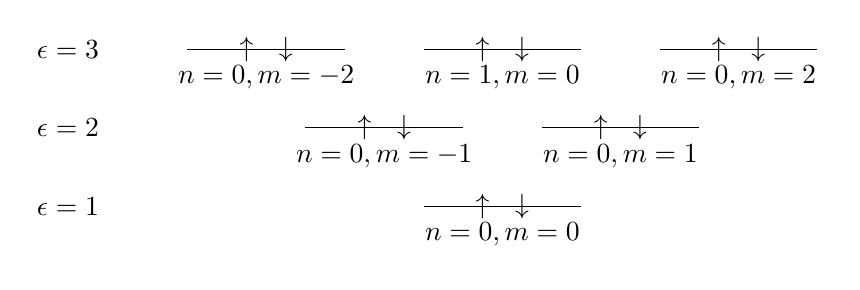
\begin{tikzpicture}
                        \begin{scope}
                            \foreach \i in {1, 2, 3} {
                                \draw(-1, \i - 1) node[anchor=east]
                                {$\epsilon = \i$};
                            }

                            % Highest energy level
                            \foreach \i in {0, 3, 6} {
                                \draw (\i, 2) -- (\i + 2, 2);
                                \node at (\i + 0.75, 2) {$\uparrow$};
                                \node at (\i + 1.25, 2) {$\downarrow$};
                            }
                            \node[below, inner sep=.2cm] at (1, 2)
                            {$n = 0, m = -2$};
                            \node[below, inner sep=.2cm] at (4, 2)
                            {$n = 1, m = 0$};
                            \node[below, inner sep=.2cm] at (7, 2)
                            {$n = 0, m = 2$};

                            % Middle energy level
                            \foreach \i in {1.5, 4.5} {
                                \draw (\i, 1) -- (\i + 2, 1);
                                \node at (\i + 0.75, 1) {$\uparrow$};
                                \node at (\i + 1.25, 1) {$\downarrow$};
                            }
                            \node[below, inner sep=.2cm] at (2.5, 1)
                            {$n = 0, m = -1$};
                            \node[below, inner sep=.2cm] at (5.5, 1)
                            {$n = 0, m = 1$};

                            % Lowest energy level
                            \draw (3, 0) -- (5, 0);
                            \node at (3 + 0.75, 0) {$\uparrow$};
                            \node at (3 + 1.25, 0) {$\downarrow$};
                            \node[below, inner sep=.2cm] at (4, 0)
                            {$n = 0, m = 0$};
                        \end{scope}
                    \end{tikzpicture}
                \end{center}
                \caption{In this plot we can see the energy degeneracy of the lowest
                three energy levels in the two-dimensional quantum dot.
                Each arrow representes a spin up or a spin down state with the
                quantum numbers $n$ and $m$ as listed below.
                This pattern goes on indefinitly with the addition of one bar
                (two oscillators) per level.}
                \label{fig:tdho-energy-levels}
            \end{figure}


        \subsubsection{Mapping the quantum numbers to a single value}
            When working with second quantized operators, we distinguish single
            particle functions in a Slater determinant by a single index.
            Including spin in the two-dimensional harmonic oscillator
            eigenstates we have to deal with three quantum numbers $n$, $m$, and
            $m_s$ per state.
            We are thus interested in finding a mapping $(n, m) \mapsto p$ and
            the inverse mapping $p \mapsto (n, m)$.\footnote{%
                The spin quantum number is easiest to deal with in the end as we
                can double each dimension in every matrix and label all odd or
                even indices by a spin direction.
            }
            Due to the degeneracy of the eigenenergies such a mapping will not
            be unique.
            We thus have to decide in advance how we should count the basis
            states.
            In this thesis we choose the convention that we start from the
            lowest energy level and move up by counting from left to right.
            Tabulating \autoref{fig:tdho-energy-levels} we get the table shown
            in \autoref{tab:tdho-mapping}.
            In \autoref{alg:nm-to-p} we give a sketch of the algorithm we use to
            compute $(n, m) \mapsto p$. We show the inverse algorithm in
            \autoref{alg:p-to-nm}.

            Using the aforementioned mapping we can find indices $p$ such that
            \begin{align}
                \ket{\psi_{nm}} \mapsto \ket{\psi_p},
            \end{align}
            and similarly for the eigenenergies
            \begin{align}
                \epsilon_{nm} \mapsto \epsilon_{p}.
            \end{align}

            \begin{table}
                \centering
                \caption{In this table we show an example of how our mapping
                convention will index the states shown in
                \autoref{fig:tdho-energy-levels}.}
                \renewcommand{\arraystretch}{1.3}
                \begin{tabular}{@{}lll@{}}
                    \toprule
                    $\epsilon_{nm}$ & $(n, m)$ & $p$ \\
                    \midrule
                    $1$ & $(0, 0)$ & $0$ \\
                    $2$ & $(0, -1)$ & $1$ \\
                    $2$ & $(0, 1)$ & $2$ \\
                    $3$ & $(0, -2)$ & $3$ \\
                    $3$ & $(1, 0)$ & $4$ \\
                    $3$ & $(0, 2)$ & $5$ \\
                    \bottomrule
                \end{tabular}
                \label{tab:tdho-mapping}
            \end{table}

            \begin{algorithm}
                \inputpython{implementation/quantum-systems/get_index_p.py}{0}{35}
                \caption{In this algorithm we describe how we can find $(n, m)
                \mapsto p$ relatively quick without having to tabulate all
                maps.}
                \label{alg:nm-to-p}
            \end{algorithm}

            \begin{algorithm}
                \inputpython{implementation/quantum-systems/get_indices_nm.py}{0}{48}
                \caption{In this algorithm we sketch how we can find $p \mapsto
                (n, m)$, i.e., the inverse of \autoref{alg:nm-to-p}.}
                \label{alg:p-to-nm}
            \end{algorithm}

        \subsubsection{Computing the dipole moments}
            The matrix elements of the dipole moment of the two-dimensional
            harmonic oscillator quantum dot is given by
            \begin{align}
                \vf{d}_{ij}
                \equiv \mel{i}{\positionvec}{j},
            \end{align}
            where we get a dipole moment for each coordinate in $\vf{r}$. As
            we've expressed the single particle functions in polar coordinates,
            but wish to express the dipole moments in a cartesian coordinate
            system, we have to compute the two integrals
            \begin{align}
                \vf{d}_{ij}
                &= \vf{i}\mel{i}{\position}{j}
                + \vf{j}\mel{i}{\position[y]}{j}
                = \vf{i}\mel{i}{r \cos(\phi)}{j}
                + \vf{j}\mel{i}{r \sin(\phi)}{j},
                \label{eq:dipole_elements}
            \end{align}
            where $\vf{i}$ and $\vf{j}$ are the unit vectors along the $x$- and
            $y$-axis respectively.
            Using \autoref{eq:eigenstate-tdho} we are able to find analytical
            expressions for the angular integral.
            The radial integral must be evaluated from $0$ to $\infty$, but
            lucikly SymPy \cite{sympy} handles this for us.
            Note that we use the notation $i \mapsto (n_i, m_i)$ from the
            mapping algorithms described above. We then get the following
            integrals
            \begin{align}
                \mel{i}{r \cos(\phi)}{j}
                &= N^{*}_{n_i m_i} N_{n_j m_j}
                \mathcal{R}_{ij}
                \mathcal{C}_{ij},
                \\
                \mel{i}{r \sin(\phi)}{j}
                &= N^{*}_{n_i m_i} N_{n_j m_j}
                \mathcal{R}_{ij}
                \mathcal{S}_{ij},
            \end{align}
            where no summation is implied in the index labels.
            The integrals are given by
            \begin{gather}
                \mathcal{R}_{ij}
                =
                \int_{0}^{\infty} \dd r r^2
                R_{n_i m_i}^{*}(r) R_{n_j m_j}(r),
                \label{eq:radial-integral-tdho}
                \\
                \mathcal{C}_{ij}
                =
                \int_{0}^{2\pi}
                \dd \phi
                \cos(\phi)
                \Phi_{m_i}^{*}(\phi)
                \Phi_{m_j}(\phi),
                \label{eq:cos-integral-tdho}
                \\
                \mathcal{S}_{ij}
                =
                \int_{0}^{2\pi}
                \dd \phi
                \sin(\phi)
                \Phi_{m_i}^{*}(\phi)
                \Phi_{m_j}(\phi).
                \label{eq:sin-integral-tdho}
            \end{gather}
            We solve the radial integral using SymPy \cite{sympy}.
            We start by constructing the radial functions $R_{n_i m_i}(r)$.
            This is done by the Python function shown in
            \autoref{alg:radial-function-tdho}, where the mapping from $i
            \mapsto (n_i, m_i)$ is done by \autoref{alg:p-to-nm}.
            \begin{algorithm}
                \inputpython{implementation/quantum-systems/spf_radial_function.py}{0}{10}
                \caption{Python function constructing the radial functions from
                the \autoref{eq:radial-function-tdho}.}
                \label{alg:radial-function-tdho}
            \end{algorithm}
            Having constructed the two radial functions we can perform the
            integraion using the function in \autoref{alg:radial-integral-tdho}.
            \begin{algorithm}
                \inputpython{implementation/quantum-systems/radial_integral.py}{0}{7}
                \caption{Python function performing the radial integral in
                \autoref{eq:radial-integral-tdho} using SymPy \cite{sympy} to
                evaluate the integral from $r \in [0, \infty)$.}
                \label{alg:radial-integral-tdho}
            \end{algorithm}

            The two angular integrals in \autoref{eq:cos-integral-tdho} and
            \autoref{eq:sin-integral-tdho} have closed form solutions which we
            derive.
            Starting with \autoref{eq:cos-integral-tdho} we can write
            \begin{align}
                \mathcal{C}_{ij}
                &=
                \int_{0}^{2\pi}
                \dd \phi
                \cos(\phi)
                \exp[-i\Delta m_{ij} \phi],
            \end{align}
            where we've defined the difference in the angular quantum number by
            \begin{align}
                \Delta m_{ij} \equiv m_i - m_j.
                \label{eq:diff-m-tdqd}
            \end{align}
            and we have that $\Delta m_{ij} \in \mathbb{Z}$.
            The closed form solution to this integral is
            \begin{align}
                \mathcal{C}_{ij}
                &= \brak{
                    \frac{\exp[-i\Delta m_{ij} \phi]}{1 - (\Delta m_{ij})^2}
                    \brak{
                        -i\Delta m_{ij} \cos(\phi)
                        + \sin(\phi)
                    }
                }_{0}^{2\pi}
                = 0,
                \label{eq:dipole-x-tdqd}
            \end{align}
            if $\Delta m_{ij} \neq \pm 1$.
            For the case when $\Delta m_{ij} = \pm 1$ we solve the easier
            integral
            \begin{align}
                \mathcal{C}_{ij}
                &=
                \int_{0}^{2\pi}
                \dd \phi
                \cos(\phi) \exp[\mp i\phi]
                \\
                &=
                \int_{0}^{2\pi}
                \dd \phi
                \para{
                    \cos^2(\phi)
                    \mp i\cos(\phi)\sin(\phi)
                }
                = \pi.
            \end{align}
            % TODO: Discuss the connection to the allowed dipole transitions in
            % a harmonic oscillator.
            For the sine integral in \autoref{eq:sin-integral-tdho} we have
            \begin{align}
                \mathcal{S}_{ij}
                &=
                \int_{0}^{2\pi}
                \dd\phi
                \sin(\phi)
                \exp[-i\Delta m_{ij} \phi].
            \end{align}
            The closed form solution of this integral is similar to the form for
            the cosine-integral.
            Again we look at the situation when $\Delta m_{ij} \neq \pm 1$
            initially.
            \begin{align}
                \mathcal{S}_{ij}
                &= \brak{
                    \frac{\exp[-i\Delta m_{ij} \phi]}{1 - (\Delta m_{ij})^2}
                    \brak{
                        -i\Delta m_{ij} \sin(\phi)
                        + \cos(\phi)
                    }
                }_{0}^{2\pi}
                = 0.
                \label{eq:dipole-y-tdqd}
            \end{align}
            For $\Delta m_{ij} = \pm 1$ we get
            \begin{align}
                \mathcal{S}_{ij}
                &=
                \int_{0}^{2\pi}
                \dd\phi
                \sin(\phi)
                \exp[\mp i\phi]
                \\
                &=
                \int_{0}^{2\pi}
                \dd\phi
                \para{
                    \sin(\phi)\cos(\phi)
                    \mp i\sin^2(\phi)
                }
                = \mp i\pi.
            \end{align}
            The results for the angular integrals yields the selection rules for
            the dipole approximation for the two-dimensional harmonic
            oscillator.
            Unless $\Delta m_{ij} = \pm 1$, the transition between the states is
            not allowed in the dipole approximation, i.e., the integral
            vanishes.
            % TODO: Write the full expression for the dipole elements.
            % TODO: Add plot of the dipole moments.


        \subsubsection{Computing the Coulomb elements}
            Having found the basis functions and the elements of the one-body
            hamiltonian, we are left with the task of finding the two-body
            elements from the Coulomb interaction.
            Luckily, there exists an analytic formula finding these elements for
            the two-dimensional harmonic oscillator in polar coordinates.
            This formula is shown in appendix A in the article
            \citetitle{anisimovas1998energy} by
            \citeauthor{anisimovas1998energy} \cite{anisimovas1998energy}.
            Note that \citeauthor{anisimovas1998energy} interchanges the indices
            in the ket-part of their two-body integrals as opposed to our
            convention. That is, in our notation we would write
            \begin{align}
                \mel{ij}{\twohamil}{kl}
                &=
                \int\dd x_1\dd x_2
                \psi_{i}^{*}(x_1) \psi_{j}^{*}(x_2)
                \twoten
                \psi_{k}(x_1)\psi_{l}(x_2)
                \equiv
                \mel{ij}{\twohamil}{lk}_{AM},
            \end{align}
            where $ \bra{ij}\twohamil\ket{lk}_{AM}$ is the convention used by
            \citeauthor{anisimovas1998energy}.
            There are two significant symmetries included in the calculation of
            the two-body elements.
            The first occurs as the Hamiltonian is spin-independent and the
            second comes from the azimuthal quantum number $m$.
            This can be expressed as
            \begin{align}
                \mel{ij}{\twohamil}{kl}
                = \delta_{\sigma_i \sigma_k} \delta_{\sigma_j \sigma_l}
                \int\dd \vf{r}_1\dd \vf{r}_2
                \psi_{i}^{*}(\vf{r}_i) \psi_{j}^{*}(\vf{r}_2)
                \twoten
                \psi_{k}(\vf{r}_1)\psi_{l}(\vf{r}_2),
            \end{align}
            where the symmetry that $m_i + m_j = m_k + m_l$ is baked into the
            integral.
            The formula for computing the integral
            \begin{align}
                \mathcal{I}^{ij}_{kl}
                =
                \int\dd \vf{r}_1\dd \vf{r}_2
                \psi_{i}^{*}(\vf{r}_1) \psi_{j}^{*}(\vf{r}_2)
                \twoten
                \psi_{k}(\vf{r}_1)\psi_{l}(\vf{r}_2),
            \end{align}
            is rather involved and we've pushed it to
            \autoref{app:coulomb-elements}.


    \subsection{Two-dimensional double well quantum dot}
        Another interesting system to explore is the double well quantum dot,
        i.e., a quantum dot with a finite barrier in the potential trap.
        Building the barrier on top of the two-dimensional harmonic oscillator
        lets us reuse much of the machinery from the previous section.
        There are a multitude of ways to create a confining double well
        potential.
        In the following we'll be focusing on a double well with a sharp
        boundary for the barrier in either $x$- or $y$-direction.
        The one-body Hamiltonian of the double well with the barrier in the
        $x$-direction is given by
        \begin{align}
            \onehamil
            &=
            \frac{\momentum^2}{2m}
            + \half m \omega^2 \position[r]^2
            + \half m \omega^2 \para{
                \frac{1}{4} l^2 - l\abs{\position}
            }.
            \label{eq:one-body-2ddw}
        \end{align}
        % TODO: Give motivation for the shape of the double-well.
        % Discuss the constant term.
        In \autoref{eq:one-body-2ddw} we recognize the two first terms as the
        kinetic energy and the harmonic oscillator confining potential.
        Instead of finding an analytical expression for the full one-body
        Hamiltonian, as we did for the harmonic oscillator, we'll instead use
        the single-particle functions in \autoref{eq:eigenstate-tdho} as trial
        wave functions and use the variational method to find as good an
        estimate as possible to the underlying exact eigenpair.
        The one-body matrix elements can then be found from
        \begin{align}
            \oneten^{p}_{q}
            &= \epsilon_{p}\delta^{p}_{q}
            + \half m \omega^2\mel{p}{\para{
                \frac{1}{4} l^2 - l \abs{\position}
            }}{q}
            \\
            &= \epsilon_{p}\delta^{p}_{q}
            + \frac{1}{8} m \omega^2 l^2 \delta^{p}_{q}
            - \half m \omega^2 l \mel{p}{\abs{\position}}{q},
        \end{align}
        where we have used the mapping $(n, m) \to p$ from
        \autoref{alg:nm-to-p} described above and where
        the eigenenergies $\epsilon_p$ are given by
        \autoref{eq:eigenenergy-tdho}.
        The two first terms give a shifted harmonic oscillator potential, viz.
        \begin{align}
            \epsilon_p' = \epsilon_p + \frac{1}{8} m \omega^2 l^2.
        \end{align}
        The last term is the double well barrier and resembles the dipole matrix
        elements from \autoref{eq:dipole_elements} except for the absolute
        value.
        We rewrite the potential barrier in polar coordinates by
        \begin{gather}
            \abs{x} = r\abs{\cos(\phi)}, \\
            \abs{y} = r\abs{\sin(\phi)},
        \end{gather}
        where we've included the barrier in $y$-direction for the sake of
        generality.
        We can thus compute the barrier integrals using the eigenstates from the
        harmonic oscillator.
        \begin{gather}
            \mel{p}{\abs{\position}}{q}
            =
            N^{*}_{n_p m_p} N_{n_q m_q}
            \mathcal{R}_{pq} \tilde{\mathcal{C}}_{pq},
            \\
            \mel{p}{\abs{\position[y]}}{q}
            =
            N^{*}_{n_p m_p} N_{n_q m_q}
            \mathcal{R}_{pq} \tilde{\mathcal{S}}_{pq},
        \end{gather}
        where the normalization and the radial integral is the same as for the
        dipole moment in the harmonic oscillator system.
        Note again that no summation is implied in the indices for the
        integrals.
        The only difference is the absolute value on the periodic functions in
        the polar integrals.
        These integrals are given by
        \begin{gather}
            \tilde{\mathcal{C}}_{pq}
            =
            \int_{0}^{2\pi} \dd \phi
            \abs{\cos(\phi)}
            \Phi^{*}_{m_p}(\phi)
            \Phi_{m_q}(\phi),
            \\
            \tilde{\mathcal{S}}_{pq}
            =
            \int_{0}^{2\pi} \dd \phi
            \abs{\sin(\phi)}
            \Phi^{*}_{m_p}(\phi)
            \Phi_{m_q}(\phi).
        \end{gather}
        For $k \in \mathbb{Z}$ and $\Delta m_{pq} \equiv m_p - m_q$, the
        solution to the cosine integral is given by
        \begin{align}
            \tilde{\mathcal{C}}_{pq}
            =
            \frac{4}{1 - (\Delta m_{pq})^2}
            \begin{cases}
                0 & \Delta m_{pq} = 2k + 1, \\
                1 & \Delta m_{pq} = 4k, \\
                -1 & \Delta m_{pq} = 4k + 2,
            \end{cases}
        \end{align}
        and for the sine integral we get
        \begin{align}
            \tilde{\mathcal{S}}_{pq}
            &=
            \frac{4}{1 - (\Delta m_{pq})^2}
            \begin{cases}
                0 & \Delta m_{pq} = 2k + 1, \\
                1 & \Delta m_{pq} = 2k.
            \end{cases}
        \end{align}
        For a full derivation, see \autoref{app:barrier-integrals}.

        Having constructed the full one-body Hamiltonian matrix $\onemat$, we
        diagonalize and find the variationally optimized eigenvectors $\vf{C}$.
        We can now use the coefficients to transform to the new double-well
        basis.
        That is, we construct the single-particle functions
        \begin{align}
            \ket{\psi_{\alpha}} = C^{p}_{\alpha}\ket{\phi_p},
        \end{align}
        where we label the double-well single-particle functions by
        $\ket{\psi_{\alpha}}$ with greek indices to distinguish from the known
        harmonic oscillator single-particle functions $\ket{\phi_p}$.
        Stated as an eigenequation for the double-well one-body Hamiltonian
        \begin{gather}
            \onehamil \ket{\psi_{\alpha}}
            = \varepsilon_{\alpha} \ket{\psi_{\alpha}}
            \implies
            \onehamil C^{q}_{\alpha} \ket{\phi_q}
            = \varepsilon_{\alpha} C^{q}_{\alpha} \ket{\phi_q},
        \end{gather}
        where we've inserted the known single-particle functions along with the
        coefficients.
        The eigenenergy $\varepsilon_{\alpha}$ is the eigenenergy of the
        double-well single-particle functions.
        Projecting onto the harmonic oscillator basis, we find a generalized
        eigenvalue equation.
        \begin{gather}
            \bra{\phi_{p}}\onehamil\ket{\phi_q} C^{q}_{\alpha}
            = \varepsilon_{\alpha} C^{q}_{\alpha} \braket{\phi_{p}}{\phi_{q}}.
        \end{gather}
        Recalling that the harmonic oscillator basis is orthonormal and
        inserting the matrix elements for the one-body Hamiltonian we are left
        with
        \begin{align}
            \oneten^{p}_{q} C^{q}_{\alpha}
            = \delta^{p}_{q} C^{q}_{\alpha} \varepsilon_{\alpha}
            = C^{p}_{\alpha} \varepsilon_{\alpha}.
        \end{align}
        Solving this generalized eigenvalue equation yields the coefficient
        matrix, $\vf{C} \in \mathbb{C}^{L\times L}$, and the eigenenergy matrix
        $\vfg{\varepsilon} = \diag(\varepsilon_1, \dots, \varepsilon_L)$, where
        $L$ is the number of harmonic oscillator basis functions.
        Having found the coefficient matrix we can transform the two-body
        elements from the harmonic oscillator basis to the double-well basis by
        \begin{align}
            \bra{\psi_{\alpha} \psi_{\beta}}
            \twohamil
            \ket{\psi_{\gamma} \psi_{\delta}}
            = {C^{p}_{\alpha}}^{*}
            {C^{q}_{\beta}}^{*}
            \bra{\phi_{p} \phi_{q}}
            \twohamil
            \ket{\phi_{r} \phi_{s}}
            C^{r}_{\gamma}
            C^{s}_{\delta}.
        \end{align}
        The same procedure can also be used on other matrix elements defined in
        the harmonic oscillator basis. For example, the dipole matrix elements
        yields
        \begin{align}
            \bra{\psi_{\alpha}}
            \vf{d}
            \ket{\psi_{\beta}}
            = {C^{p}_{\alpha}}^{*}
            \bra{\phi_{p}}
            \vf{d}
            \ket{\phi_{q}}
            C^{q}_{\beta}.
        \end{align}

        \subsubsection{Quality of the transformed single-particle functions}
            As the harmonic oscillator basis in no way is a complete basis
            covering enough of the Hilbert space in order to accurately describe
            the double-well basis, we need to make a choice on how many basis
            functions we deem ``good enough''.
            % TODO: This sentence needs rephrasing.


    \section{Atomic and molecular systems}
        Having discussed systems of quantum dots, or so-called ``artificial
        atoms'', we will now focus on actual atomic and molecular systems.
        As stated at the start of this chapter we make use of existing
        libraries to construct atomic and molecular basis sets.
        We will therefore touch briefly on the topic of atomic and molecular
        basis sets as much of the work therein will be treated as a black box.
        The molecular electronic one-body Hamiltonian in the Born-Oppenheimer
        approximation is given by \cite{basis-sets, hochstuhl2014time}
        \begin{align}
            \onehamil_i
            = -\half \nabla^2_i
            - \frac{Z_A}{\abs{\vfg{R}_A - \vfg{r}_i}}
        \end{align}
        where atomic units are assumed.
        Note that we sum over all nuclei $A$.
        Here we've left out the internuclear repulsion and the Coulomb
        interaction.
        Furthermore, in the Born-Oppenheimer approximation we treat the nuclei
        as being frozen and therefore ignore the kinetic energy contribution of
        the nuclear core.

        Now, perhaps not surprisingly the exact solution of the full molecular
        Hamiltonian\footnote{%
            Even in the Born-Oppenheimer approximation.
        } is a far fetched goal for all but the smallest systems to say the
        least.
        Similar to the procedure we did for the double-well in
        \autoref{subsec:tddw} we can solve the molecular Hamiltonian in an
        approximate basis set.
        We can then diagonalize the one-body Hamiltonian and express the
        matrix elements in this new basis.
        We can also use Hartree-Fock to improve on our approximate basis, but
        both of these methods rely on an approximate basis set which are
        complete to be fully exact.
        This is seldom the case due to computational limitations.
        As a consequence a lot of effort in the quantum chemistry field has been
        put into the construction of efficient and good basis sets.
        We will in this thesis use the following basis sets:
        \begin{itemize}
            \item The minimal Slater-type orbital (STO-$k$G) basis sets
                \cite{sto-3g, helgaker-molecular}.
                Here $k$ denotes the number of Gaussian primitive functions used
                in a single basis function.
            \item The split-valence ($X$-$YZ$g) basis sets \cite{x-yzg,
                helgaker-molecular}.
                Here $X$ denotes the number of primitive Gaussian functions for
                the core basis functions.
                The $Y$ and $Z$ tells us that there are two sets of basis
                functions with $Y$ and $Z$ basis functions respectively, for the
                valence orbitals.
            \item The correlation-consistent polarized valence (cc-pV$X$Z) basis
                sets \cite{cc-pVXZ, helgaker-molecular}.
                These basis sets are better tuned for post Hartree-Fock methods.
                The $X$ parameter decides the number of functions for the
                valence electrons, e.g., $D$ for double-zeta, $T$, for
                triple-zeta, etc.
            \item The augmented correlation-consistent (aug-cc-pV$X$Z) basis
                sets \cite{aug-cc-pVXZ, helgaker-molecular}.
                The cc-pV$X$Z basis sets are designed for ground state
                calculations, but are inferior when it comes to describing
                excited states.
                The aug-cc-pV$X$Z basis functions alleviates some of this by
                incuding diffuse functions for the outer valence electrons
                \cite{helgaker-molecular}.
                The parameter $X$ is the same as in the case of the cc-pV$X$Z
                basis set.
        \end{itemize}
        To reuse the basis sets from PySCF \cite{pyscf} and Psi4 \cite{psi4}
        we've created a class \pyth{CustomSystem} which allows us to build a
        \pyth{QuantumSystem}-class by manually setting the matrix elements.
        We can thus ask PySCF and Psi4 to use their well-optimized methods to
        generate basis sets and reuse these in our solvers.
        In this thesis we will only use basis sets from PySCF and we therefore
        only describe the interface towards this library.
        We've created three interface functions denoted
        \pyth{construct_pyscf_system_ao}, \pyth{construct_pyscf_system_rhf}, and
        \pyth{construct_pyscf_system} which sets up a \pyth{CustomSystem} of
        atomic orbitals, restricted molecular orbitals, and unrestricted
        molecular orbitals respectively.
        The two latter methods use the restricted and unrestricted Hartree-Fock
        solvers of PySCF.
        There are two main input parameters to these functions and that is
        \pyth{molecule} and \pyth{basis}.
        The former is a string describing the atom or molecule.
        In case of an atom it is enough to write the chemical symbol for the
        atom, e.g., \pyth{"he"} for Helium.
        For molecules the coordinates of the atoms contained in the system must
        be included.
        In the case of a diatomic molecules we can then specify a bond distance
        along a specific axis, e.g., \pyth{f"h 0 0 0; h 0 0 1.2"} for a
        \ch{H2}-molecule with the bond distance $1.2$ specified in atomic units
        along the $z$-axis.
        The basis strings share the same format as discussed above, e.g., to
        specify the usage of aug-cc-pVDZ, we pass in the string
        \pyth{"aug-ccpvdz"} as the basis.


    \section{Particle density}
        \label{sec:particle-density}
        From \autoref{subsec:particle-density} we know how to compute the
        one-body particle density once we have found the one-body density matrix
        from a specific solver.
        For variational methods where the dual state of $\ket{\phi_p}$ is the
        adjoint $\bra{\phi_p}$ we can use the expression in
        \autoref{eq:particle-density}.
        However, as we are focusing much of our work on the bi-variational
        formulation of coupled-cluster we will implement the more general
        particle-density calculation
        \begin{align}
            \densityten(x)
            = \tilde{\phi}_{q}(x)
            \densityten^{q}_{p}
            \phi_p(x),
        \end{align}
        where $\tilde{\phi}_q(x)$ is the bi-variational dual state of
        $\phi_p(x)$.
        For the Hartree-Fock methods and configuration-interaction solvers we
        choose $\tilde{\phi}_q(x) = \phi^{*}_q(x)$ and we have recovered the
        original expression for the particle density as seen in
        \autoref{eq:particle-density}.
        In \autoref{alg:particle-density} we've included the code used to
        compute the particle density given a one-body density matrix denoted
        \pyth{rho_qp}, and the set of orbitals \pyth{bra_spf} and \pyth{ket_spf}
        as the bra- and ket-states respectively.
        We let the first index (the rows) of the orbital arrays denote the
        orbital index $p$, $q$, etc, whereas the remaining indices define the
        evaluation of the function on a $d$-dimensional grid $x \in
        \mathbb{C}^{d}$.
        \begin{algorithm}
            \begin{python}
def compute_particle_density(rho_qp, bra_spf, ket_spf):
    rho = np.zeros(ket_spf.shape[1:], dtype=ket_spf.dtype)
    spf_slice = slice(0, ket_spf.shape[0])

    for _i in np.ndindex(rho.shape):
        i = (spf_slice, *_i)
        rho[_i] += np.dot(bra_spf[i], np.dot(rho_qp, ket_spf[i]))

    return rho
            \end{python}
            \caption{In this listing we've added a function computing the
            particle density on an arbitrary grid that the orbitals are
            represented on.}
            \label{alg:particle-density}
        \end{algorithm}

    \section{Change of basis}
        \label{sec:change-of-basis}
        Much of what we do in this thesis is related to basis transformations.
        Either by diagonalization of the one-body Hamiltonian, an initial
        Hartree-Fock calculation, or in the orbital rotations in the
        non-orthogonal and orbital-adaptive coupled-cluster methods.
        A basis transformation can in general be represented by
        \begin{align}
            \ket*{\psi_p} = C_{\alpha p} \ket*{\phi_{\alpha}},
            \label{eq:spf-basis-change}
        \end{align}
        where we use greek indices to denote a basis of $K$ orbitals
        $\brac{\phi_{\alpha}}$ and latin letters for the basis of $L$
        transformed orbitals $\brac{\psi_p}$, and where $\vfg{C} \in
        \mathbb{C}^{K\times L}$ is a complex matrix with the coefficients.

        Having found the coefficient matrix $\vfg{C}$ we can change basis for
        all the existing matrix elements stored in the
        \pyth{QuantumSystem}-class.
        We will also here assume for the sake of generality that the dual state
        $\tilde{\psi}_p(x)$ not necessarily is the adjoint of $\psi_p(x)$.
        This means that
        \begin{align}
            \bra*{\tilde{\psi}_p}
            = \tilde{C}_{p \alpha}\bra*{\phi_{\alpha}},
            \label{eq:spf-dual-basis-change}
        \end{align}
        where we assume that the dual states in the underlying orbital basis are
        the adjoint states.
        Take extra note of the ordering of the indices in the coefficients in
        the dual basis transformation.
        In the case of adjoint states we have the familiar $\tilde{C}_{p \alpha}
        = C^{*}_{\alpha p}$.
        From the list of contents in \pyth{QuantumSystem} at the top of this
        chapter, we have three types of basis transformations that we need to
        support to fully change our system.
        We need to be able to change basis for one- and two-body matrix
        elements, and for the single-particle functions.

        We denote arbitrary one-body matrix elements of the one-body matrix
        $\vfg{\oneten}$ in the original orbital basis by
        \begin{align}
            \oneten_{\alpha \beta}
            \equiv
            \mel*{\phi_{\alpha}}{\onehamil}{\phi_{\beta}}.
        \end{align}
        Transforming to the new basis set we have
        \begin{gather}
            \tilde{\oneten}_{pq}
            = \mel*{\tilde{\psi}_p}{\onehamil}{\psi_q}
            =
            \tilde{C}_{p\alpha}
            \oneten_{\alpha \beta}
            C_{\beta q}
            \\
            \implies
            \tilde{\vfg{\oneten}}
            = \tilde{\vfg{C}}
            \vfg{\oneten}
            \vfg{C},
        \end{gather}
        where $\tilde{\vfg{\oneten}}$ is the transformed one-body elements.
        An implmentation of the change of basis for the one-body elements is
        shown in \autoref{alg:transform-one-body-elements}.
        In the case of the dipole moments we store these as an array of one-body
        elements, one for every dimension, which means that we need to transform
        each axis using the algorithm in
        \autoref{alg:transform-one-body-elements}.
        \begin{algorithm}
            \begin{python}
def transform_one_body_elements(h, c, c_tilde=None):
    if c_tilde is None:
        c_tilde = c.conj().T

    return c_tilde @ h @ c
            \end{python}
            \caption{This function changes basis for the one-body matrix
            elements given a coefficient matrix \pyth{c} and an optional dual
            coefficient matrix \pyth{c_tilde}.}
            \label{alg:transform-one-body-elements}
        \end{algorithm}
        For the two-body elements we denote the elements by
        \begin{align}
            \twoten^{\alpha\beta}_{\gamma\delta}
            \equiv
            \mel*{\phi_{\alpha}\phi_{\beta}}{
                \twohamil
            }{\phi_{\gamma}\phi_{\delta}},
        \end{align}
        where we do not care if the elements are antisymmetric or not as it does
        not change the basis transformation.
        The transformation can now be done by
        \begin{align}
            \tilde{\twoten}^{pq}_{rs}
            = \mel*{\phi_p\phi_q}{
                \twohamil
            }{\phi_r\phi_s}
            = \tilde{C}_{p\alpha}
            \tilde{C}_{q\beta}
            \twoten^{\alpha\beta}_{\gamma\delta}
            C_{\gamma r}
            C_{\delta s}.
        \end{align}
        In \autoref{alg:transform-two-body-elements} we demonstrate the function
        which changes the basis for the two-body elements.
        We make use of temporary storage of a two-body matrix \pyth{_u} which
        lowers the cost of the basis transformation from $\mathcal{O}(L^8)$ to
        $\mathcal{O}(L^5)$.
        \begin{algorithm}
            \begin{python}
def transform_two_body_elements(u, c, c_tilde=None):
    if c_tilde is None:
        c_tilde = c.conj().T

    # abcd, ds -> abcs
    _u = np.tensordot(u, c, axes=(3, 0))
    # abcs, cr -> absr -> abrs
    _u = np.tensordot(_u, c, axes=(2, 0)).transpose(0, 1, 3, 2)
    # abrs, qb -> arsq -> aqrs
    _u = np.tensordot(_u, c_tilde, axes=(1, 1)).transpose(
        0, 3, 1, 2
    )
    # pa, aqrs -> pqrs
    _u = np.tensordot(c_tilde, _u, axes=(1, 0))

    return _u
            \end{python}
            \caption{This function changes the basis of the two-body elements
            given a coefficient matrix \pyth{c} and an optional dual matrix
            \pyth{c_tilde}.}
            \label{alg:transform-two-body-elements}
        \end{algorithm}
        For the single-particle functions the basis transformation is performed
        by the equations in \autoref{eq:spf-basis-change} and
        \autoref{eq:spf-dual-basis-change} where the states are projected on a
        grid.
        We represent all the single-particle states as an $d + 1$-dimensional
        array, where the first axis denotes which single-particle state we are
        looking at, and the $d$-remaining axes denotes the grid.
        In \autoref{alg:transform-spfs} we show the member function of
        \pyth{QuantumSystem} for changing the single-particle state basis.
        \begin{algorithm}
            \begin{python}
class QuantumSystem:
    # Code removed for clarity

    def change_basis_spf(self, c, c_tilde=None):
        if c_tilde is not None:
            # In case of bi-orthogonal basis sets, we create an
            # extra set of single-particle functions for
            # the bra-side
            self._bra_spf = self.np.tensordot(
                c_tilde,
                self._spf.conj()
                if self._bra_spf is None else self._bra_spf,
                axes=((1), (0)),
            )

        self._spf = self.np.tensordot(
            c, self._spf, axes=((0), (0))
        )
            \end{python}
            \caption{Here we list the member function in \pyth{QuantumSystem}
            that transforms the single-particle states given a coefficient
            matrix \pyth{c} and an optional dual matrix \pyth{c_tilde}.
            The single-particle states are denoted \pyth{self._spf} and
            \pyth{self._bra_spf} in case of a dual state that is not the adjoint
            state.}
            \label{alg:transform-spfs}
        \end{algorithm}


    \section{Spin-doubling}
        The basis sets we are exploring are always formulated as spatial
        orbitals without any spin component.
        Furthermore, we look at spin-independent Hamiltonians for the most
        part\footnote{%
            We explore a spin-dependent laser field to some extent as will be
            demonstrated in the results.
        } and a restricted solution can be used where we incorporate the spin by
        reusing the doubly occupied orbitals.
        We will use this to some extent for the restricted Hartree-Fock solver
        which will be discussed in \autoref{subsec:rhf}.
        However, most of the methods we've implemented make no assumption on the
        spin-orbitals other than there being two spin-components, and therefore
        allow general spin-orbitals as discussed in
        \autoref{subsec:restrictions-on-spin-orbitals}.
        This means that after we've created our basis sets, we include spin by
        making the system doubly degenerate in each orbital.

        The ordering of the spin-orbitals are important as some solvers
        exploit the spin-degeneracy and therefore need to know how the
        spin-orbitals are ordered.
        We've chosen a solution which is far from optimal, but which is
        reasonable as long as we have an even number of particles with the same
        amount of particles in each spin-direction.
        We use the convention that orbitals are ordered in an increasing order
        based on their single-particle eigenenergy\footnote{%
            This is the ordering that is returned by NumPy when diagonalizing
            the one-body Hamiltonian.
        }.
        We then double the length of each orbital axis in the single-particle
        functions,\footnote{%
            Except for the grid axes.
        } the one-body- and two-body Hamiltonians, and all other matrix
        elements.
        Next we repeat each orbital twice so that even indices corresponds to a
        certain spin-direction and odd indices to the other direction.
        We are able to achieve this quite succintly using the Kronecker-product
        and slicing in NumPy.
        In \autoref{alg:spin-doubling-spf} we demonstrate a snippet which adds
        spin to a set of orbitals defined on an arbitrary grid.
        \begin{algorithm}
            \begin{python}
class QuantumSystem:
    # Code removed for clarity

    def change_to_spin_orbital_basis(self, anti_symmetrize=True):
        # Code removed for clarity

        if not self._spf is None:
            new_shape = [
                self._spf.shape[0] * 2, *self._spf.shape[1:]
            ]

            spf = self.np.zeros(
                tuple(new_shape), dtype=self._spf.dtype
            )
            spf[::2] += self._spf
            spf[1::2] += self._spf

            self._spf = spf
            assert self._spf.shape[0] == self.l
            \end{python}
            \caption{Spin-doubling of the single-particle functions.}
            \label{alg:spin-doubling-spf}
        \end{algorithm}
        For the one-body elements we use the function listed in
        \autoref{alg:spin-doubling-one-body}.
        The two-body elements requires us to do some more work as the Kronecker
        product gets applied to the two last indices of the array.
        We also want the product to be applied to pairwise indices that interact
        in the two-body integrals.
        This requires some transposing of the elements, and is shown in
        \autoref{alg:spin-doubling-two-body}.
        \begin{algorithm}
            \begin{python}
def add_spin_one_body(h):
    return np.kron(h, np.eye(2))
            \end{python}
            \caption{Function adding spin to one-body matrix elements, that is,
            matrices.}
            \label{alg:spin-doubling-one-body}
        \end{algorithm}
        \begin{algorithm}
            \begin{python}
def add_spin_two_body(_u):
    u = _u.transpose(1, 3, 0, 2)
    u = np.kron(u, np.eye(2))
    u = u.transpose(2, 3, 0, 1)
    u = np.kron(u, np.eye(2))
    u = u.transpose(0, 2, 1, 3)

    return u
            \end{python}
            \caption{Function adding spin to the two-body elements.}
            \label{alg:spin-doubling-two-body}
        \end{algorithm}

        A more general solution -- and which should be implemented in the future
        -- is to create spin-blocks with each spin-direction following each
        other as this allows for an unequal number of particles in each
        spin-direction.
        This is the solution that needs to be taken for the unrestricted
        Hartree-Fock method when changing basis.

    \section{Time-evolution operators}
        The only time-evolution operators used in this thesis are dipole lasers
        in the length gauge.
        We've implemented this by allowing \pyth{QuantumSystem} to have a
        pointer to a \pyth{TimeEvolutionOperator}-class, where \pyth{LaserField}
        is a subclass.
        The \pyth{LaserField}-class takes in the parameter \pyth{laser_pulse}
        and an optional \pyth{polarization_vector}.
        The former parameter is the electric field of the laser including the
        envelope function, whereas the latter defines which axis to polarize
        along.
        By default the polarization vector is set along the $x$-axis, that is,
        the first axis.
        Note that \pyth{QuantumSystem} so far does not have a charge which means
        that for negative charge either the pulse or the polarization vector
        needs to incorporate this sign.
        Both \pyth{laser_pulse} and \pyth{polarization_vector} can be constants
        or functions of a single parameter; time.
        We restrict our attention to a constant linear polarization, but we use
        time-dependent laser pulses.
        To specify a laser pulse, the user creates a function or a class with a
        \pyth{__call__}-method which takes in a single parameter as time.
        This function should return the electric field at the given time
        including the envelope function.
